\documentclass[letterpaper,11pt,twoside]{article}
\usepackage{amsmath,amssymb,amsfonts,amsthm}
\usepackage[margin=1.0in]{geometry}
\usepackage{fancyhdr, lastpage}
\usepackage[pdftex]{graphicx}
\usepackage{hyperref}
\hypersetup{
    colorlinks,
    citecolor={black},
    linkcolor={black},
    urlcolor={black},
    bookmarksnumbered,
    pdfstartview={FitH},
    pdfpagemode={UseOutlines},
    pdftitle={Project Report - Distributed Query Processing},
    pdfauthor={Larry Bowers, James Bradwell, Evan Dickinson, Bhadresh Patel, and Lewis Pearson},
    pdfsubject={CS 453 Project Report}
}

\setlength{\parskip}{0.5ex}
\pagestyle{fancy}
\setlength{\headheight}{14.0pt}
\fancyhead{}
\fancyfoot{}
\fancyhead[RO,RE] {Project Report: \emph{Distributed Query Processing}}
\fancyfoot[LO,LE] {CS 453: Project 4}
\fancyfoot[RO,RE] {Page \thepage\ of \pageref{LastPage}}
\renewcommand{\headrulewidth}{0.5pt}
\renewcommand{\footrulewidth}{0.5pt}

\begin{document}

%%%%%%%%%% Title Page %%%%%%%%%%%%%%%%%%%%%%%%%%%%%%%%%%%%%%%%%%%%%%%%%%%%%%%%%%
\begin{titlepage}
   \begin{center}
       {\Large \textbf{Project Report}}\\[0.5cm]
       {\Large \textbf{CS 453: Project 4}}\\[3.0cm]

       {\rule{\linewidth}{0.5mm}} \\[0.5cm]
       {\Huge \textbf{Distributed Query Processing}}\\[0.4cm] 
       {\rule{\linewidth}{0.5mm}} \\[2.0cm]

       \textbf{Larry Bowers}\\
       \texttt{killergift@wsu.edu}\\[0.5cm]
       \textbf{James Bradwell}\\
       \texttt{jebradwell@gmail.com}\\[0.5cm]
       \textbf{Evan Dickinson}\\
       \texttt{evan13579b@wsu.edu}\\[0.5cm]
       \textbf{Bhadresh Patel}\\
       \texttt{bhadresh@wsu.edu}\\[0.5cm]
       \textbf{Lewis Pearson}\\
       \texttt{lewis\_pearson@wsu.edu}\\[0.5cm]

       \vfill
       Washington State University Vancouver\\
       December 05, 2010
   \end{center}
\end{titlepage}

\begin{abstract}
The main goal of this project is to implement the user interface and the distributed query processing component of the Search Engine over multiple Amazon EC2 nodes using the PageRank and Indexes generated by previous project.
\end{abstract}

\section{Overview}

\begin{figure}[htbp]
 \centering
 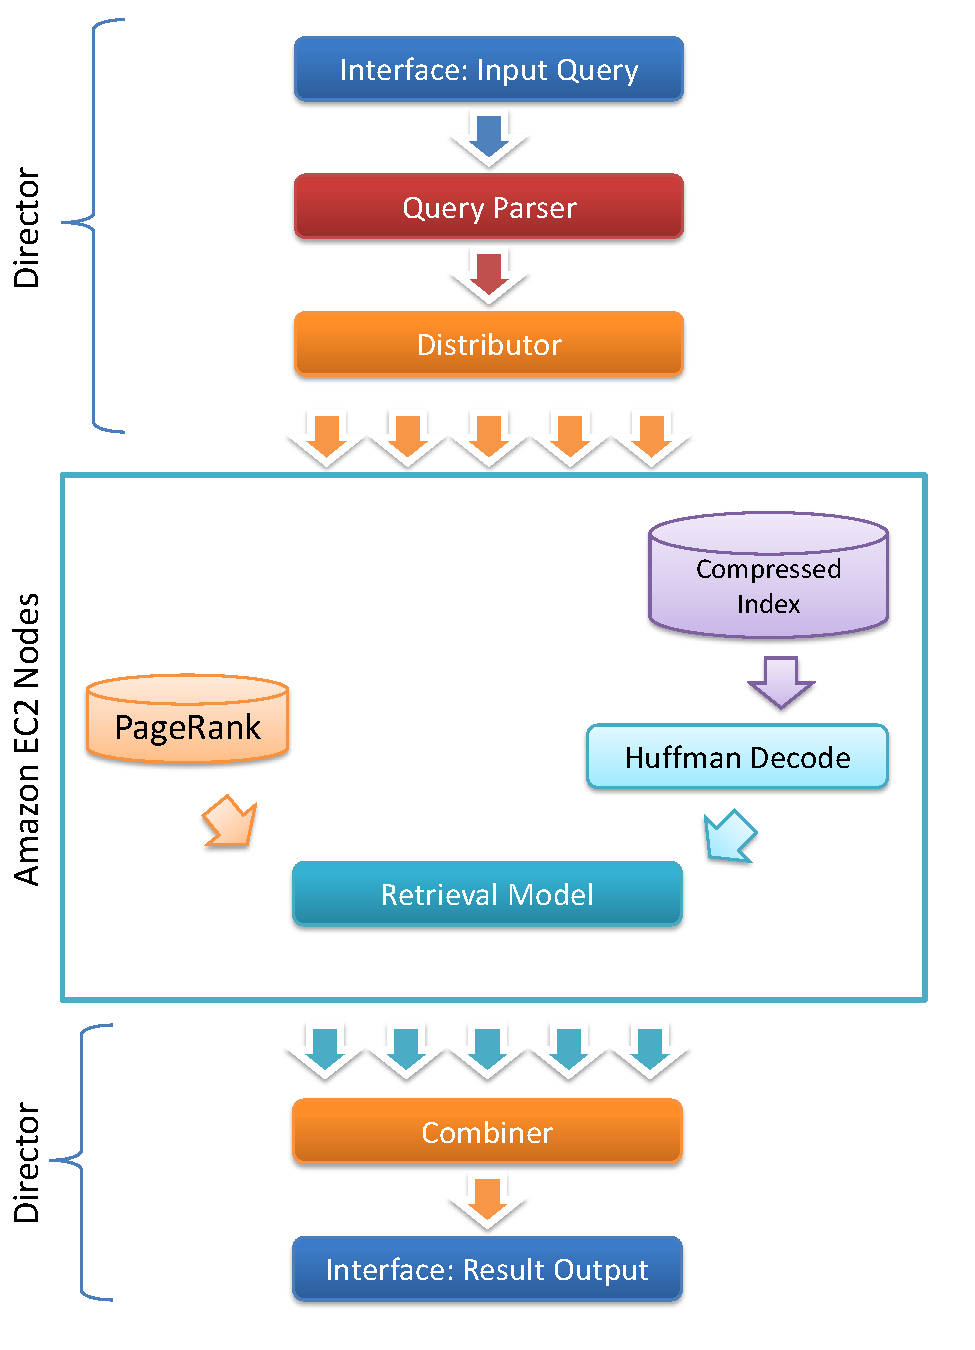
\includegraphics[trim=0.0in 0.00in 0.0in 0.0in, clip, page=1]{Architecture.pdf}
 \caption{Architecture Overview}
 \label{fig:Architecture}
\end{figure}

In this project, our goal is to implement distributed query processing component of the search engine. In previous projects, we already crawled documents, generated indexes, and calculated PageRank. Distributed query processing component utilities these information and perform user's query evaluation over multiple nodes. Figure~\ref{fig:Architecture} shows  architecture for distributed query processing. The user interface takes query input from the user and sends to the query parser. Query parser validates and parses the given query and hand off to distributer. Distributer, then connects to each index server and executes the given query. Index server finds ranked document list for the given query and sends back to distributer. Distributer merges the retrieved results and sends to the user interface, which is then displayed to the user.  

\section{Interface}

\subsection{Query Input}

\subsection{Result Output}

\section{Distributed Evaluation}

The distributed evaluation is done using six Amazon EC2 nodes as shown in figure~\ref{fig:Architecture}. One of the nodes is called director, that is responsible for hosting the user interface, execute search on all index server, combine the results, and then return the ranked list of documents to user interface. Processing of the query given by the user interface is done in simple client-server model, where index server is a simple daemon process that is started once and the distributer is client that connects to each index server when query is executed.

\subsection{Index Server}

The index server is a simple daemon process that is started and listens on socket for incoming query request. When the index server is started it load various information into the memory first and then waits for the incoming request. It loads PageRank, Index file, and pid\_map.dat files during initialization. The startup process takes indexfile name as an argument; \emph{i.e.}, which index file to use on the particular node. Thus, for each query request it only calls retrieval model to calculate relevance score using pre-loaded information in the memory. The query request contains two information: (i) Retrieval Model to use, and (ii) parsed and validated user's query. Based on the given retrieval model, index server calls the appropriate model's code to get ranked list of documents. Once the results are retrieved, they are sent back to the distributor. 

\subsection{Distributer}

Distributer is a client program, that connects to each index server, sends the query given by the user interface. It then waits for the results, collects results form all index servers and merge them. The merged results are then sorted based on relevance score and sent back to the UI based on the requested page number. Distributer creates multiple processes or threads to connect to each index server, thus it executes queries in parallel on each index server. 

Based on the query terms, distributer first finds which index server needs to be called. Since index files are sorted and split across index servers, any particular term would be available one index server only. This way we can optimize for number of processes distributer needs to create and avoid unnecessary search to any index server. 

\section{Index Compression}

\subsection{Huffman Encoding}
The first decision our group made about this feature is whether or not to consider each doc number as an atom or each character. We chose characters as atoms for simplicity and because we were unsure about how choosing numbers as atoms would scale.

To facilitate huffman encoding a class was created that stored the information needed to encode and decode for a particular document set. The class also had the methods needed to do the encoding and decoding.

To set up huffman encoding, the index files were stripped of all the terms plus the first separator because the terms were not to be encoded.

A code was then created with createCode.py on the stripped index files to get a proper encoding for the document set.

The result of creating the code was a huffman coder object that had the data and methods needed to encode and decode that document set. The object was pickled and saved into a file called `huffmanCode'.

The index files were then processed into maps and pickled. Two maps were created for each index, one that had compressed values and the other non-compressed. The maps were actually maps of maps where the first level had a `type' key saying whether the data was compressed or uncompressed and a `data' key whose corresponding value was a map containing all the terms with the string that contains their counts information.

The compressed index had to be pickled so that the count string wouldn't create ambiguities when compressed into a binary form. If the terms were not separated from the compressed count string the compressed count string could have been compressed into a newline followed by what looks like a term making one think that the part that is compressed follows the illusionary newline and false-term.

Since the compressed index had to be pickled, the normal one was also pickled for consistency and also so that the pickled map could hold information about whether or not it was compressed.

Example index:
ant:4:(434,1)

ant becomes key with corresponding value: \texttt{4:(434,1)} in non-compressed version and \texttt{\#\$\^\$} in compressed version.

\subsection{Huffman Decoding}
The retrieval model class contains a `coder' member which is read into the class from the `huffmanCode' file in the data directory at initialization.

This coder member is stored and sent to the score calculation functions to be used when retrieving term counts. The score calculation functions pass the coder to the getTermContent function which returns the terms based on the index type. The index is also passed to the getTermContent function and its `type' key is used to identify if it is compressed or not. If it is compressed the compressed count string is decompressed using the coder and the resulting decompressed string is then parsed into a map containing the counts for the term overall and in each document.

If the type of the index is `uncompressed' the index will have already had its count string parsed into an appropriate map which is returned by getTermContent.

The compression ratio for each count string was generally a little under 2.

For index-0 the size in memory of each map was ~460000 bytes compressed and ~740000 non-compressed (before each non-compressed entry is parsed into a map after which the non-compressed size would be much larger). The original file size was ~570000 bytes.

Time-wise no significant time increase was noticed. To test the time taking by decoding I ran a test that decoded the value corresponding to every term in the index and for 2500 files the result was 4 seconds.

4/2500=~1.6ms. Our average query was around 0.3 seconds or 300 ms making the decoding insignificant in comparison.

\section{Retrieval Model}

\subsection{Query Likelihood}

\subsection{BM25}

\section{Roles}
\begin{description}
  \item[Larry Bowers] User interface and query parser
  \item[James Bradwell] User interface and query parser
  \item[Evan Dickinson] Huffman encoding/decoding 
  \item[Bhadresh Patel] Distributed evaluation
  \item[Lewis Pearson] Retrieval model
\end{description}

\section{Test Environment}

For testing/production purpose, we have set up instances on Amazon EC2. The instance id of the director machine is i-5135773c which also hosts the user interface. Instance ids of five index servers are: (i) i-5335773e, (ii) i-2d357740, (iii) i-2f357742, (iv) i-29357744, and (v) i-2b357746. The source code on all instances is checked out at /home/ubuntu/dqp/. The user interface can be accessed via public DNS name of the director instance. For example, http://ec2-174-129-159-24.compute-1.amazonaws.com/ui/.

\section{Usage Guide}

\begin{itemize}
	\item Update Nodes file \texttt{dp/local.nodes} or \texttt{dp/cloud.nodes}. Change the IP address of all nodes for the appropriate environment.
	\item Start index server on each instance
\begin{verbatim}
	$ python ~/dqp/dp/server.py
\end{verbatim}
	\item Find the public DNS of the director instance \texttt{i-5135773c}. Launch the UI using public DNS, for example, http://ec2-174-129-159-24.compute-1.amazonaws.com/ui/.
\end{itemize}

\end{document}
